\section{Analysis}

\begin{figure}[htbp]
	\centering
	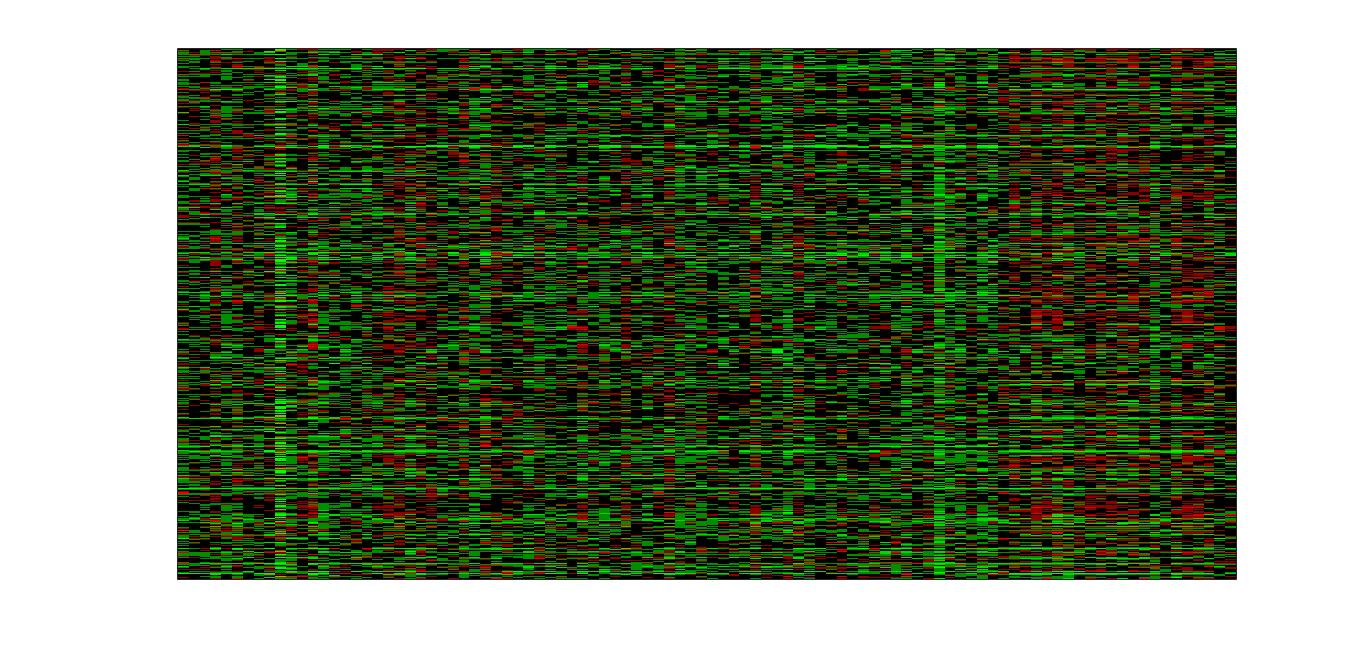
\includegraphics[width=\linewidth,height=15cm,keepaspectratio]{analisis/raw.jpg}
	\caption{Heatmap raw data}
	\label{pic:raw}
\end{figure}

\begin{figure}[htbp]
	\centering
	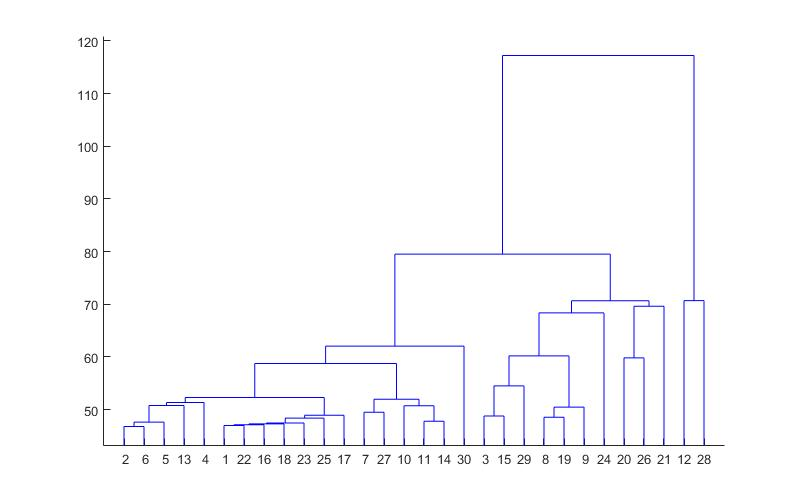
\includegraphics[width=\linewidth,height=15cm,keepaspectratio]{analisis/dendogram.jpg}
	\caption{Dendogram}
	\label{pic:dendo}
\end{figure}

\begin{figure}[htbp]
	\centering
	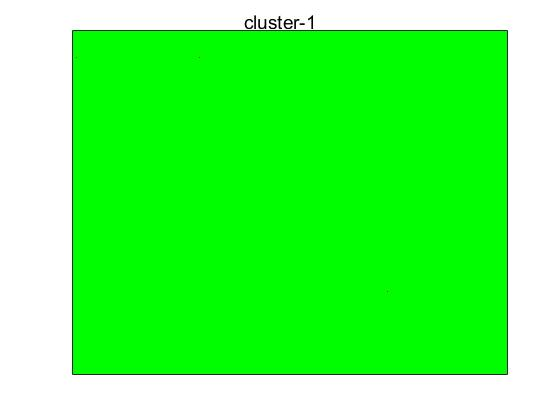
\includegraphics[width=\linewidth,height=15cm,keepaspectratio]{analisis/cluster-1.jpg}
	\caption{Heatmap cluster-1}
	\label{pic:cluster-1}
\end{figure}

\begin{figure}[htbp]
	\centering
	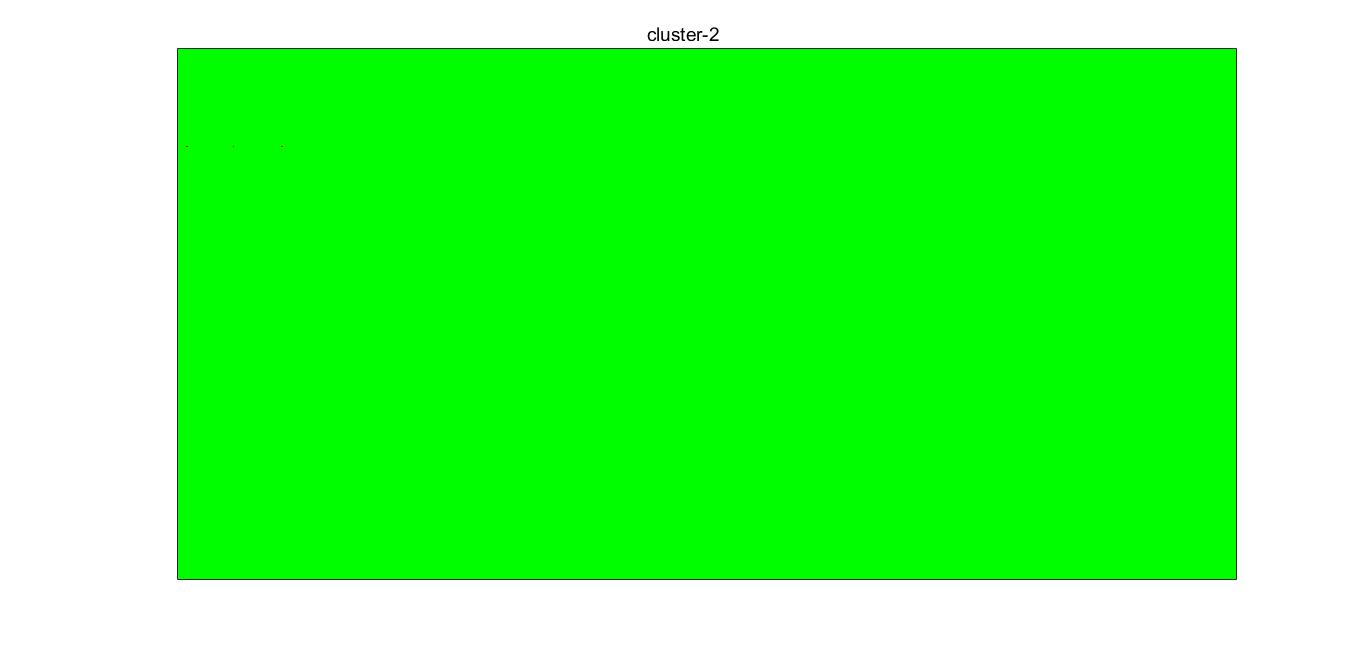
\includegraphics[width=\linewidth,height=15cm,keepaspectratio]{analisis/cluster-2.jpg}
	\caption{Heatmap cluster-2}
	\label{pic:cluster-2}
\end{figure}

\begin{figure}[htbp]
	\centering
	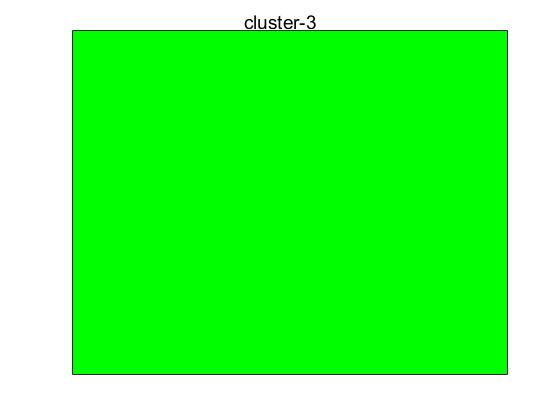
\includegraphics[width=\linewidth,height=15cm,keepaspectratio]{analisis/cluster-3.jpg}
	\caption{Heatmap cluster-3}
	\label{pic:cluster-3}
\end{figure}

\begin{figure}[htbp]
	\centering
	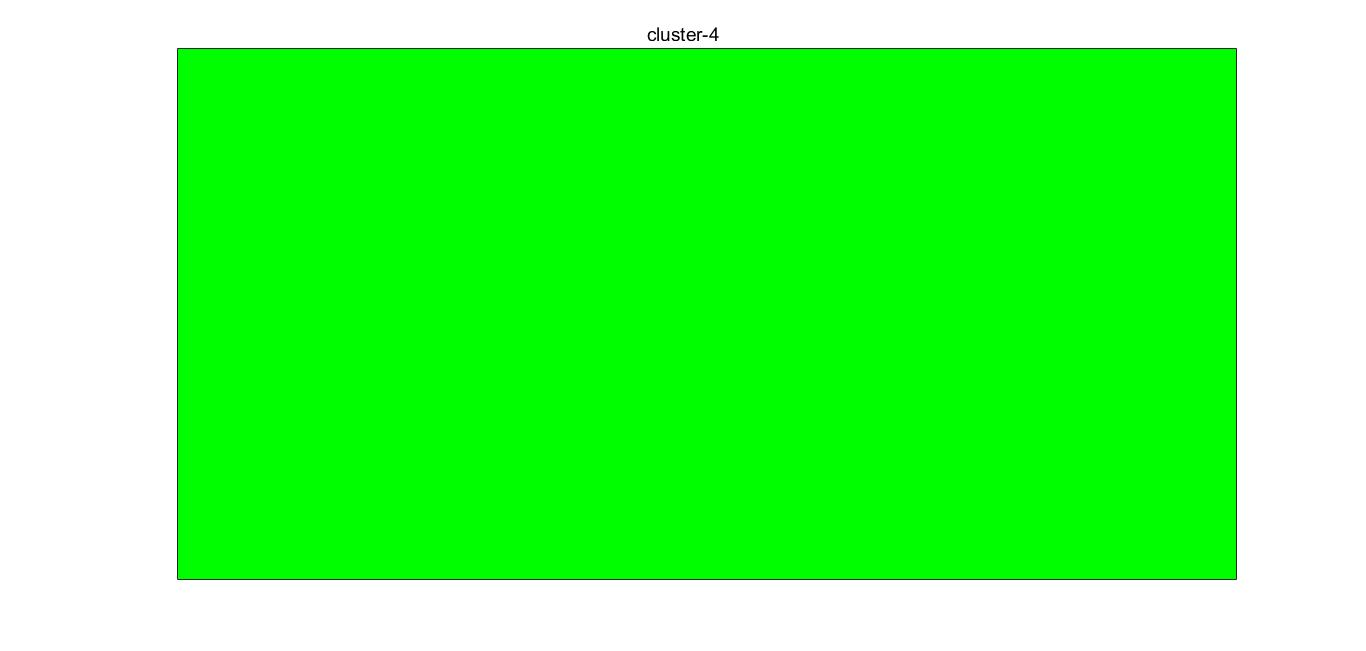
\includegraphics[width=\linewidth,height=15cm,keepaspectratio]{analisis/cluster-4.jpg}
	\caption{Heatmap cluster-4}
	\label{pic:cluster-4}
\end{figure}


\begin{figure}[htbp]
	\centering
	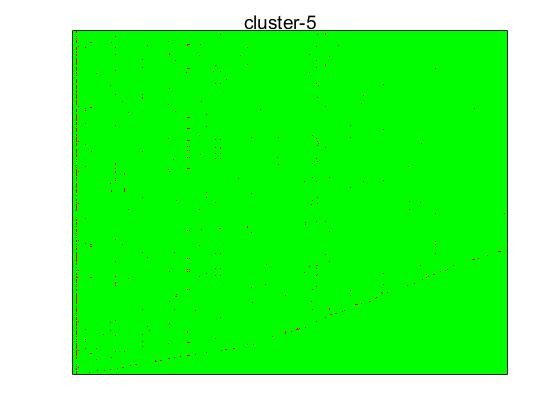
\includegraphics[width=\linewidth,height=15cm,keepaspectratio]{analisis/cluster-5.jpg}
	\caption{Heatmap cluster-5}
	\label{pic:cluster-5}
\end{figure}

from the result, can be seen that the most common gene that show up in the cluster is GO:0005515 which has function of protein binding.
